\documentclass{beamer}
\usepackage{graphicx}
\usepackage{amsmath}
\usepackage{listings}
\usepackage{xcolor}
\usepackage{helvet}
\usepackage{hyperref}
\usepackage{subcaption}

% Define colors for code and presentation theme
\definecolor{codegreen}{rgb}{0,0.6,0}
\definecolor{codegray}{rgb}{0.5,0.5,0.5}
\definecolor{codepurple}{rgb}{0.58,0,0.82}
\definecolor{themecolor}{RGB}{45, 62, 80}

% Setup for code blocks
\lstset{
  language=Python,
  basicstyle=\footnotesize\ttfamily,
  keywordstyle=\color{blue},
  commentstyle=\color{codegreen},
  stringstyle=\color{codepurple},
  numbers=left,
  numberstyle=\tiny\color{codegray},
  breaklines=true,
  showspaces=false,
  showstringspaces=false,
  showtabs=false,
  tabsize=4
}

% Beamer theme
\usetheme{Madrid}
\usecolortheme[named=themecolor]{structure}

% Title information
\title{\textbf{Predicting College Basketball Success}}
\author{Luigi Manieri}
\institute{Alma Mater Studiorum Bologna}
\date{\today}

\setbeamertemplate{footline}{%
  \leavevmode%
  \hbox{%
    \begin{beamercolorbox}[wd=.3\paperwidth,ht=2.25ex,dp=1ex,leftskip=2ex]{author in head/foot}%
      Luigi Manieri%
    \end{beamercolorbox}%
    \begin{beamercolorbox}[wd=.4\paperwidth,ht=2.25ex,dp=1ex,center]{title in head/foot}%
      Predicting College Basketball Success%
    \end{beamercolorbox}%
    \begin{beamercolorbox}[wd=.3\paperwidth,ht=2.25ex,dp=1ex,right]{date in head/foot}%
      \insertframenumber{} / \inserttotalframenumber%
    \end{beamercolorbox}%
  }%
  \vskip0pt%
}


\begin{document}

% Title slide
\begin{frame}
    \titlepage
\end{frame}

% Outline slide
\begin{frame}{Outline}
    \tableofcontents
\end{frame}

\section{Project Overview}
\begin{frame}{Project Overview}
  \begin{itemize}
    \item \textbf{Objective:} Predict whether the road team wins a game.
    \item \textbf{Dataset:} Sports match data from Kaggle competition.
    \begin{itemize}
        \item \href{https://www.kaggle.com/competitions/wfusummer2018}{https://www.kaggle.com/competitions/wfusummer2018}
    \end{itemize}
    \item \textbf{Target variable:} \texttt{Win} (1 = Road Team Wins, 0 = Loss).
  \end{itemize}
\end{frame}

% Dataset Overview
\section{Data}
\begin{frame}{Dataset Overview}
\begin{itemize}
    \item Dataset details:
        \begin{itemize}
            \item 1893 rows, 11 features, and 1 target column (Win)
            \item Numerical features: \textit{win, day, year, roadTeamPoints}
            \item Categorical features: \textit{month, weekday, time, roadTeam, locale, homeTeam, conference, OT}
        \end{itemize}
    \end{itemize}
        \begin{figure}
            \centering
            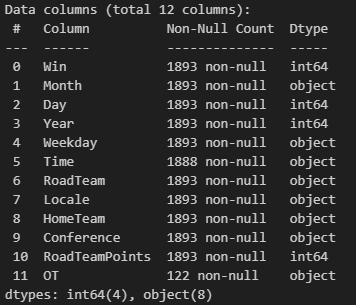
\includegraphics[width=0.35\linewidth]{images/dataset_columns.png}
            \caption{Dataset info}
            \label{fig:enter-label}
        \end{figure}
\end{frame}

% Data Exploration
\section{Data exploration}
\begin{frame}{Data Exploration}
    \begin{figure}
        \centering
        \includegraphics[width=1\linewidth]{images/dataset_head.png}
        \caption{Head of the dataset}
        \label{fig:enter-label}
    \end{figure}
    We can already see that:
    \begin{itemize}
        \item most of the features are object and need to be processed before training models
        \item some feature don't seem very informative (i.e. locale, month, day, weekday)
        \item there are some missing values (time and OT columns)
    \end{itemize}
\end{frame}

% Data Visualization
\section{Data Visualization}
\begin{frame}{Data Visualization}
    \begin{itemize}
        \item Class Balance:
            \begin{figure}
                \centering
                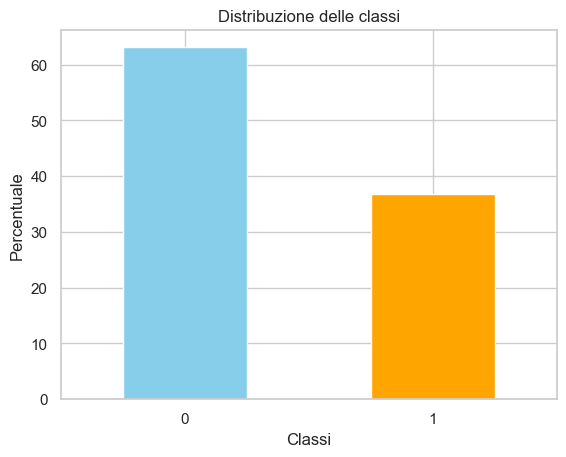
\includegraphics[width=0.75\linewidth]{images/class_balance.png}
            \end{figure}
    \end{itemize}
\end{frame}

\begin{frame}{Data Visualization}
    \begin{itemize}
        \item Correlation matrix (for numerical features):
            \begin{figure}
                \centering
                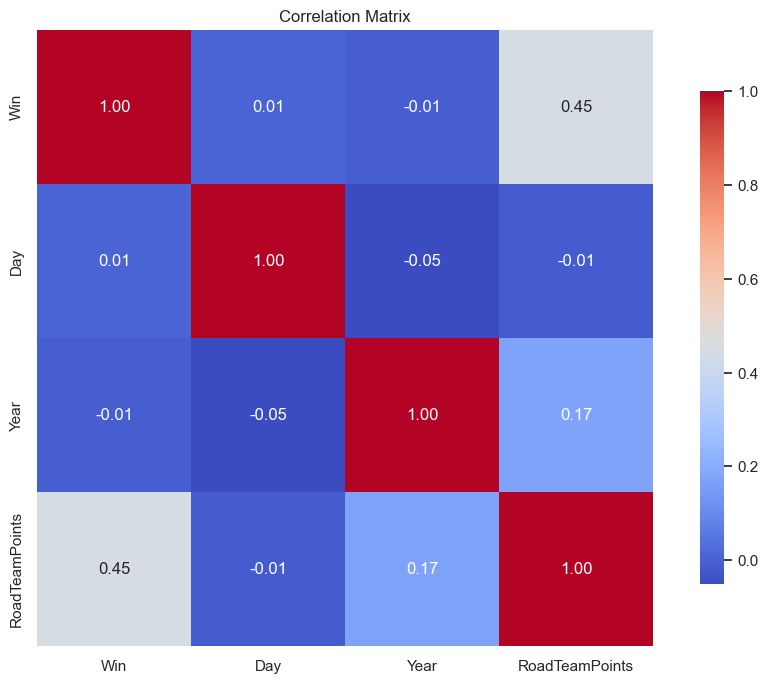
\includegraphics[width=0.75\linewidth]{images/correlation_matrix.png}
            \end{figure}
    \end{itemize}
\end{frame}

\begin{frame}{Data Visualization}
    \begin{itemize}
        \item Feature vs Target
    \end{itemize}
    \begin{figure}
        \centering
        \begin{subfigure}[b]{0.4\linewidth}
            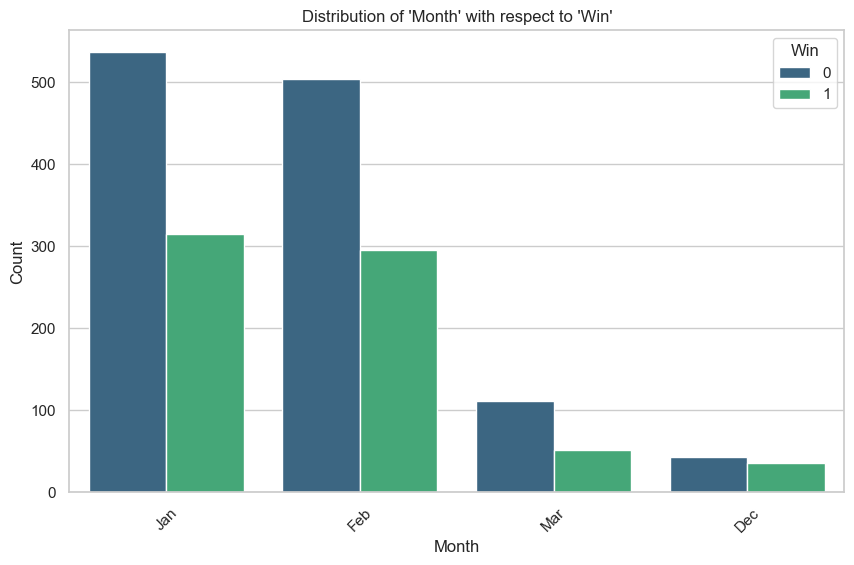
\includegraphics[width=\linewidth]{images/month_win.png}
        \end{subfigure}
        \begin{subfigure}[b]{0.4\linewidth}
            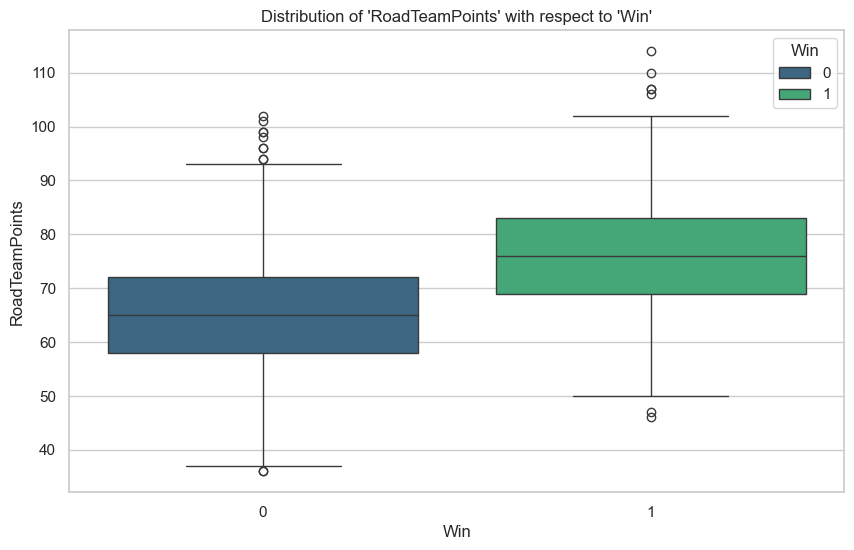
\includegraphics[width=\linewidth]{images/points_win.png}
        \end{subfigure}
        \begin{subfigure}[b]{0.4\linewidth}
            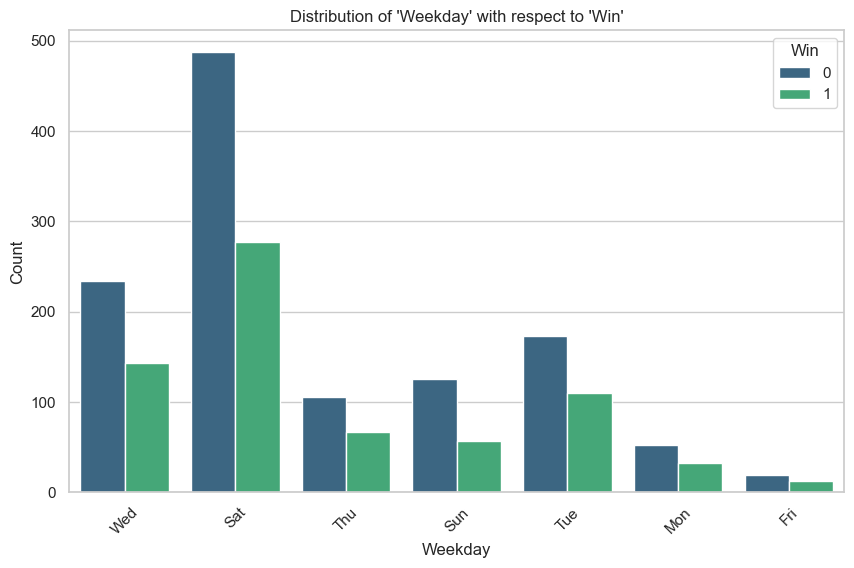
\includegraphics[width=\linewidth]{images/weekday_win.png}
        \end{subfigure}
        \begin{subfigure}[b]{0.4\linewidth}
            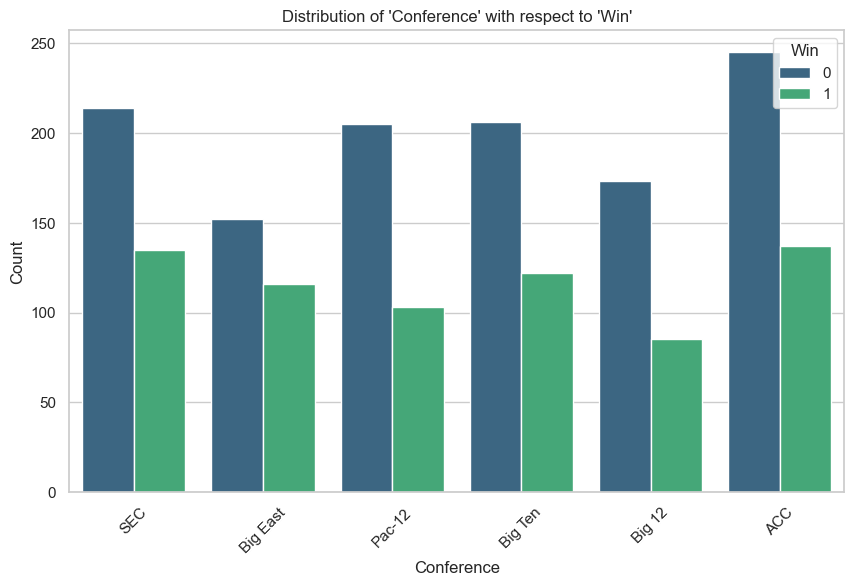
\includegraphics[width=\linewidth]{images/conference_win.png}
        \end{subfigure}
    \end{figure}
\end{frame}


% Data Preprocessing
\section{Data Preprocessing}
\begin{frame}{Data Preprocessing}
    \begin{itemize}
        \item Deal with missing values and duplicates
            \begin{itemize}
                \item in Time column \textrightarrow\  dropped
                \item in OT column \textrightarrow\  substitute with placeholder value NOT (No OverTime)
                \item duplicates \textrightarrow\  dropped
            \end{itemize}
        \item Drop unnecessary columns:
            \begin{itemize}
                \item Locale, Day, Weekday, Month
                    \begin{itemize}
                        \item I tried to encode them instead of drop \textrightarrow\  no performance gain
                    \end{itemize}
            \end{itemize}
    \end{itemize}
\end{frame}

\begin{frame}{Data Preprocessing}
    \begin{itemize}
        \item One hot encoding
        \begin{itemize}
            \item for HomeTeam and RoadTeam features
        \end{itemize}

        \item Label encoding
        \begin{itemize}
            \item for OT and Conference
        \end{itemize}

        \item MinMaxScaling:
            \begin{itemize}
                \item Year
            \end{itemize}

        \item RoadTeamPoints was not scaled in order to give it more importance
        \begin{itemize}
            \item it's the most informative feature
        \end{itemize}
    \end{itemize}
    
\end{frame}

\begin{frame}{Data Preprocessing: Processed dataset}
    \begin{figure}
        \centering
        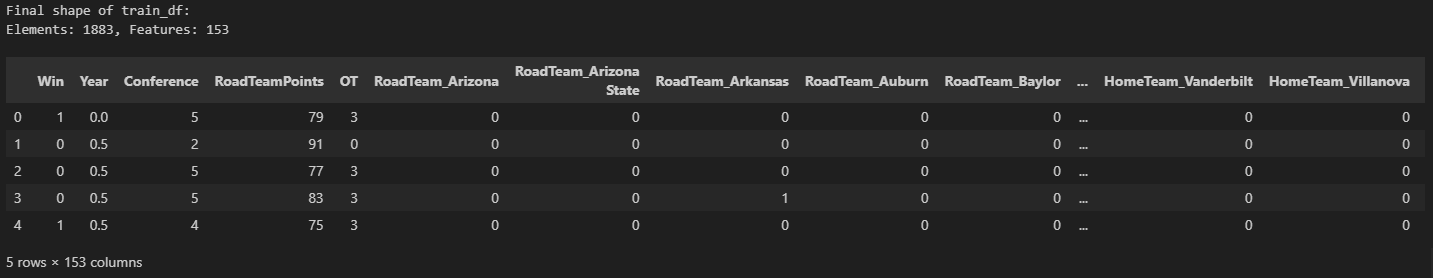
\includegraphics[width=0.9\linewidth]{images/final_dataset.png}
        \caption{Final structure of the dataset}
        \label{fig:enter-label}
    \end{figure}
\end{frame}

% Model Selection
\section{Model Training}
\begin{frame}{Data preparation and models}
    \begin{itemize}
        \item Define features X and target variable y (Win)
        \item Applying SMOTE for class balancing
        \item Dataset division: 80\% training set, 20\% test set.
        \item Measures in output: Accuracy, Recall, F1-score, ROC AUC score
        \item Models considered:
            \begin{itemize}
                \item Random Forest
                \item AdaBoost
                \item SVM
                \item XGBoost
                \item MLP
            \end{itemize}
    \end{itemize}
\end{frame}

\begin{frame}{Model training}
    \begin{itemize}
        \item Train the models with default hyperparameters
        \item Optimize them with GridSearch in order to find the best parameter configuration
            \begin{itemize}
                \item Does not always result in better performance
            \end{itemize}
    \end{itemize}
    \begin{figure}
        \centering
        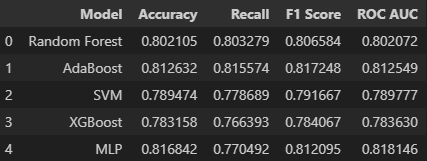
\includegraphics[width=0.5\linewidth]{images/model_results.png}
        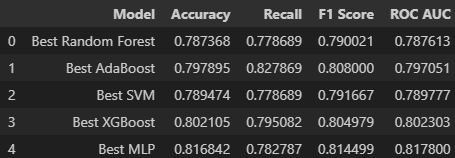
\includegraphics[width=0.5\linewidth]{images/best_model_results.png}
        \caption{Results before and after GridSearch}
        \label{fig:enter-label}
    \end{figure}
\end{frame}

% Results
\section{Models Results}
\begin{frame}{Confusion Matrix: Random Forest}
    \begin{figure}
        \centering
        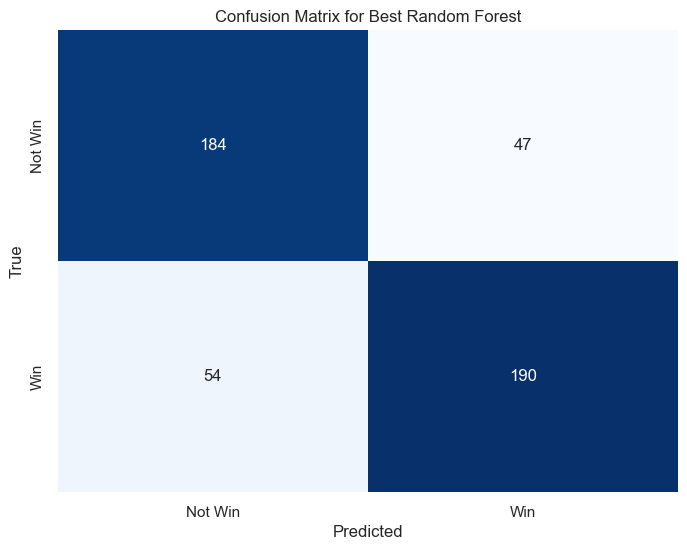
\includegraphics[width=0.7\linewidth]{images/cm_randomforest.png}
        \caption{Confusion matrix for GS-optimized Random Forest}
        \label{fig:enter-label}
    \end{figure}
\end{frame}

\begin{frame}{Confusion Matrix: AdaBoost}
    \begin{figure}
        \centering
        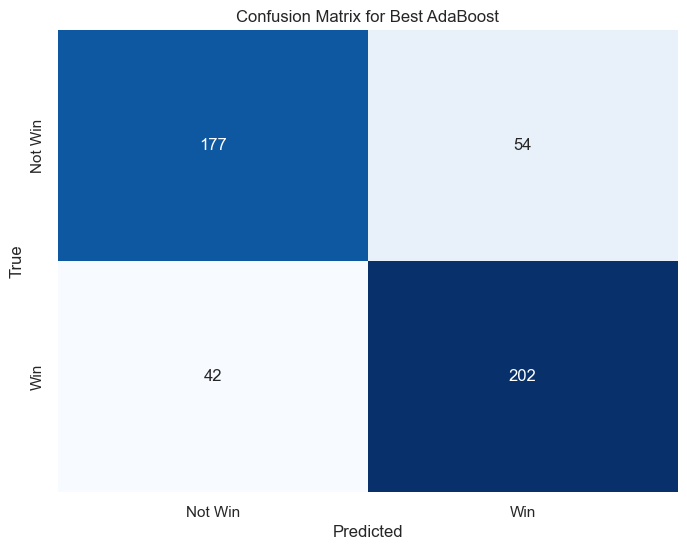
\includegraphics[width=0.7\linewidth]{images/cm_adaboost.png}
        \caption{Confusion matrix for GS-optimized AdaBoost}
        \label{fig:enter-label}
    \end{figure}
\end{frame}

\begin{frame}{Confusion Matrix: XGBoost}
    \begin{figure}
        \centering
        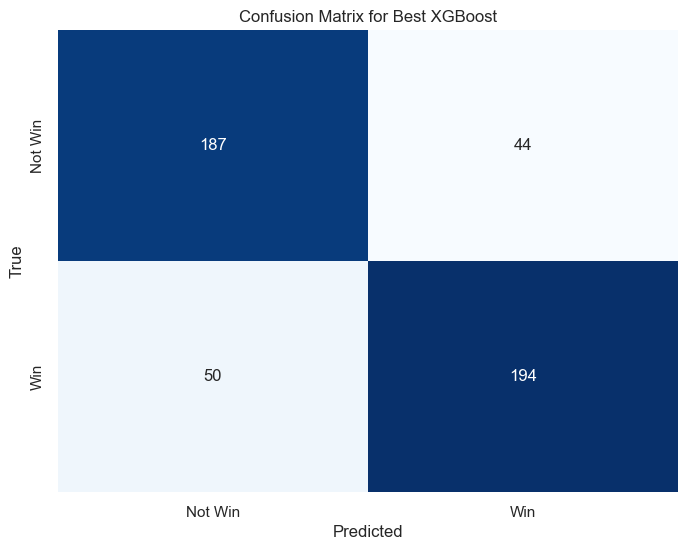
\includegraphics[width=0.7\linewidth]{images/cm_xgboost.png}
        \caption{Confusion matrix for GS-optimized XGBoost}
        \label{fig:enter-label}
    \end{figure}
\end{frame}

\begin{frame}{Confusion Matrix: SVM}
    \begin{figure}
        \centering
        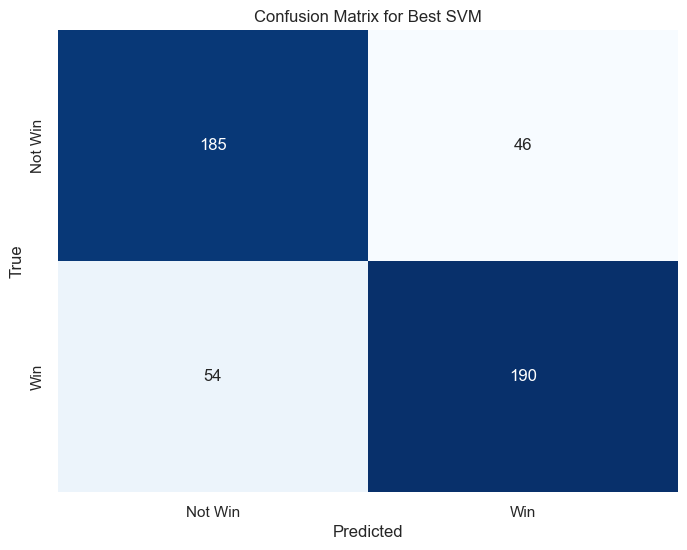
\includegraphics[width=0.7\linewidth]{images/cm_svm.png}
        \caption{Confusion matrix for GS-optimized SVM}
        \label{fig:enter-label}
    \end{figure}
\end{frame}

\begin{frame}{Confusion Matrix: MLP}
    \begin{figure}
        \centering
        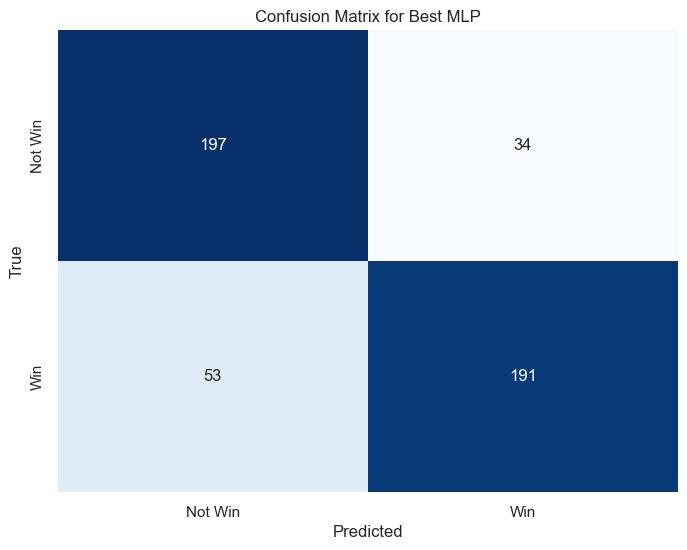
\includegraphics[width=0.7\linewidth]{images/cm_mlp.png}
        \caption{Confusion matrix for GS-optimized MLP}
        \label{fig:enter-label}
    \end{figure}
\end{frame}

% Conclusion
\section{Results Conclusions}
\begin{frame}{Results Conclusions}
    \begin{itemize}
        \item Model performance was similar across different classifiers.
        \item Grid search and hyperparameter tuning led to only marginal improvements.
        \item The most significant performance gain came from addressing class imbalance using SMOTE.
        \item This highlights that data quality and balance are more critical than model complexity.
        \item With low-quality or poorly structured data, model performance quickly reaches a ceiling - better data is the only way to raise that limit.
    \end{itemize}
\end{frame}

\begin{frame}{Results Conclusions}
    \centering
    \begin{minipage}{0.45\linewidth}
        \centering
        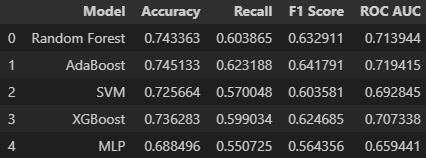
\includegraphics[width=\linewidth]{images/models_result_nosmote.png}\vspace{0.5em}
        
        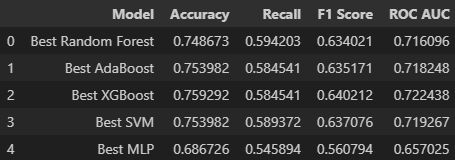
\includegraphics[width=\linewidth]{images/best_model_results_nosmote.png}
        
        \vspace{0.5em}
        \textbf{(a) No SMOTE}
    \end{minipage}
    \hspace{1cm}
    \begin{minipage}{0.45\linewidth}
        \centering
        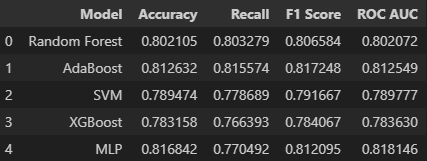
\includegraphics[width=\linewidth]{images/model_results.png}\vspace{0.5em}
        
        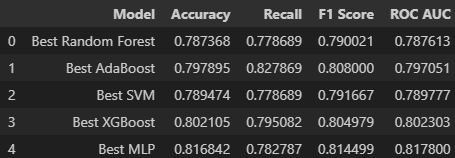
\includegraphics[width=\linewidth]{images/best_model_results.png}
        
        \vspace{0.5em}
        \textbf{(b) With SMOTE}
    \end{minipage}
\end{frame}



\end{document}